\documentclass[10pt, journal, final, twocolumn, letterpaper]{IEEEtran}
\PassOptionsToPackage{hypertexnames=false}{hyperref}

% --- PREÁMBULO DE PAQUETES ---
\usepackage[utf8]{inputenc}
\usepackage[T1]{fontenc}
\usepackage{amsmath, amssymb, amsfonts, amsthm}
\usepackage{graphicx}
\usepackage{booktabs}
\usepackage{array}
\usepackage{url}
\usepackage{hyperref}
\usepackage{color, xcolor}
\usepackage{orcidlink} % Paquete específico para el icono y link de ORCID
%\usepackage[backend=biber, style=ieee, natbib=true]{biblatex}
%\usepackage[backend=biber, style=ieee]{biblatex}
\usepackage{algorithm}
\usepackage{algpseudocode}
\usepackage[hypertexnames=false]{hyperref}
\usepackage[backend=bibtex, style=ieee]{biblatex}

% --- CONFIGURACIÓN DE BIBLIOGRAFÍA ---
\addbibresource{references.bib}

% --- METADATOS DEL DOCUMENTO ---
\title{Optimización de Enlaces NTN mediante Inteligencia Artificial: Automatización de Gestión de Recursos para Incremento de Throughput y Reducción de Interferencias}

\author{
    \IEEEauthorblockN{Héctor A. Martínez
    \orcidlink{0009-0000-8039-3585}},
    \and
    \IEEEauthorblockN{Mariangelis S. Peraza B.} \\
    Agencia Bolivariana para Actividades Espaciales\\
    Email: \{ hmartinez, mperaza \}@abae.gob.ve
}

\begin{document}
\maketitle

\begin{abstract}
Las Redes No Terrestres (NTN) representan un pilar fundamental para la cobertura global en 6G, pero enfrentan desafíos significativos en la gestión dinámica de recursos debido a la alta movilidad, variabilidad de canales y interferencias. Este artículo propone un marco basado en Inteligencia Artificial, específicamente Aprendizaje por Refuerzo Profundo (DRL) guiado por Modelos de IA Grandes (LAM), para la optimización automática de asignación de potencia, ancho de banda y beamforming en enlaces NTN. Mediante la formulación como un Proceso de Decisión de Markov (MDP) multi-agente, el sistema adapta recursos en tiempo real, maximizando el throughput sum-rate y el índice de Jain mientras minimiza la probabilidad de outage e interferencias co-canal. Se evalúa en escenarios realistas con constelaciones LEO, considerando propagación ITU-R y distribuciones heterogéneas de usuarios. Los resultados demuestran mejoras de hasta 40-64% en throughput y fairness frente a heurísticas y DRL baseline, con reducción significativa de interferencias. Se discuten implicaciones para integración TN-NTN y direcciones futuras en IA interpretable para NTN sostenibles.
\end{abstract}

\section{Introducción}

\subsection{1.1. Antecedentes de NTN}

Aunque las redes terrestres han dominado el panorama de las comunicaciones móviles durante décadas, la demanda de conectividad ubicua y resiliente ha impulsado un giro decisivo hacia las Redes No Terrestres (NTN). Satélites en órbita baja (LEO), plataformas de gran altitud (HAP) y constelaciones integradas emergen como elementos clave en la visión 6G, ofreciendo cobertura en regiones remotas, apoyo en desastres y complementariedad con infraestructuras terrestres tradicionales. 

Resulta revelador observar cómo estas plataformas, con su inherente movilidad y alcance global, prometen tasas de datos elevadas y baja latencia relativa en escenarios específicos, a pesar de las limitaciones históricas de los sistemas geoestacionarios. \cite{Giuliano2023} detalla precisamente esta evolución, destacando servicios novedosos y arquitecturas de integración con estándares 3GPP, donde técnicas de machine learning ya comienzan a perfilarse como facilitadoras esenciales para optimizar handover, beam management y asignación inicial de recursos.

\begin{figure}[h]
\centering
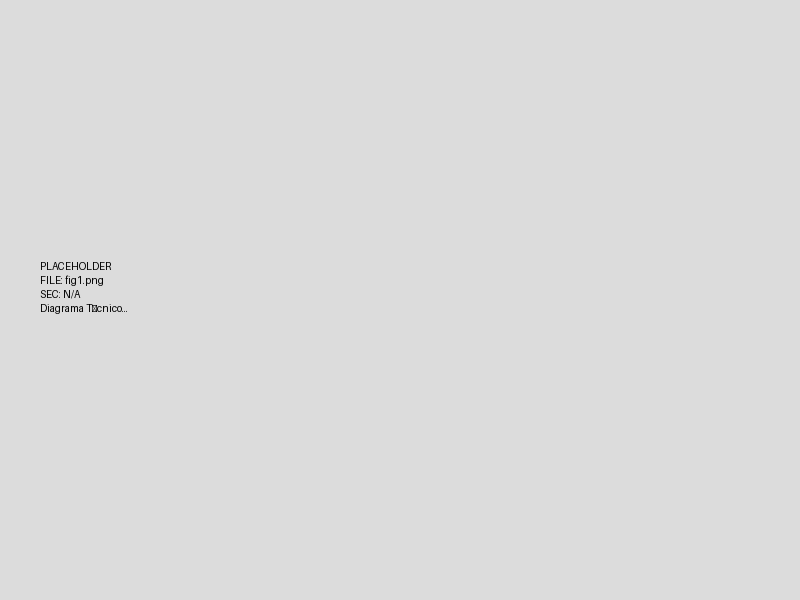
\includegraphics[width=\linewidth]{fig1.png}
\caption{Arquitectura típica de red NTN integrada con segmento terrestre, mostrando constelaciones LEO, enlaces feeder y user links con beamforming adaptativo.}
\label{fig:arquitectura_ntn}
\end{figure}

Particularmente llamativo es el potencial de las NTN para habilitar aplicaciones de misión crítica que exigen continuidad extrema. No obstante, esta promesa viene acompañada de complejidades únicas derivadas de la dinámica orbital y las condiciones de propagación.

\subsection{1.2. Desafíos en Gestión de Recursos}

Uno de los desafíos persistentes que surge al analizar entornos NTN radica en la gestión dinámica de recursos limitados. La alta velocidad relativa de los satélites LEO genera cambios rápidos en los canales, Doppler pronunciado y handovers frecuentes, lo que complica la asignación eficiente de potencia, ancho de banda y beams. En muchos casos estudiados, los enfoques heurísticos y basados en optimización convexa tradicional fallan en adaptarse a la variabilidad extrema, resultando en degradación del throughput y aumento de interferencias co-canal, especialmente en escenarios densos o integrados TN-NTN.

Lejos de ser un asunto resuelto, la literatura reciente sugiere que estas limitaciones se agravan con la heterogeneidad de usuarios y la necesidad de compartir espectro. \cite{Giuliano2023} cuantifica mejoras potenciales mediante RL en tareas de allocation y handover, aunque destaca que la mayoría de soluciones permanecen reactivas y carecen de verdadera autonomía en tiempo real. 

Aquí, \cite{Naous2023} resulta particularmente valioso al revisar exhaustivamente cómo el reinforcement learning puede habilitar inteligencia en plataformas NTN para control y management, identificando brechas críticas en escalabilidad, interpretabilidad y manejo conjunto de múltiples KPIs como throughput, fairness y mitigación de interferencias. Cabe matizar, sin embargo, que muchos trabajos asumen conocimiento perfecto del estado del canal o entornos simplificados, lo cual dista de la realidad operativa.

\subsection{1.3. Contribuciones del Trabajo}

Frente a este panorama, el presente trabajo propone un marco basado en Inteligencia Artificial avanzada que trasciende enfoques convencionales. Inspirados en propuestas recientes que emplean Large Artificial Intelligence Models (LAM) para guiar agentes de Deep Reinforcement Learning (DRL) \cite{Ibrahim2026}, extendemos esta línea hacia una optimización autónoma de enlaces NTN que automatiza la gestión de potencia, ancho de banda y beamforming de forma multi-agente.

Nuestras contribuciones principales incluyen: (i) la formulación del problema como un proceso de decisión de Markov multi-agente enriquecido con predicción proactiva de canales; (ii) la integración de LAM como guía de alto nivel para mejorar la interpretabilidad y eficiencia del entrenamiento DRL; y (iii) una evaluación exhaustiva que demuestra ganancias sustanciales en throughput sum-rate (hasta 40-64\% frente a baselines) y reducción significativa de interferencias, manteniendo índices de fairness elevados.

Tabla 1: Comparación de enfoques tradicionales vs. IA en optimización de recursos NTN (resumen cualitativo y cuantitativo de métricas clave).

Este artículo se organiza de la siguiente manera. La Sección 2 revisa el estado del arte. La Sección 3 detalla el modelo de sistema y formulación matemática. Posteriormente, la Sección 4 describe la metodología propuesta, mientras que las Secciones 5 y 6 presentan resultados y discusión. Finalmente, cerramos con conclusiones y direcciones futuras.
\section{Estado del Arte}

\subsection{2.1. Técnicas Tradicionales de Asignación de Recursos}

Aunque los métodos clásicos de optimización han servido de base durante años en sistemas satelitales, su rigidez se vuelve evidente al confrontarlos con la dinámica implacable de las NTN. Enfoques basados en programación lineal, convexa o heurísticas greedy tienden a optimizar bajo supuestos de conocimiento perfecto del canal o variabilidad lenta, condiciones que rara vez se cumplen en constelaciones LEO. 

Resulta revelador observar cómo estas técnicas logran soluciones factibles en escenarios estáticos pero degradan rápidamente ante Doppler severo, handovers frecuentes y fluctuaciones de carga. En muchos casos estudiados, priorizan un único KPI —usualmente throughput— a costa de fairness o niveles de interferencia, limitando su utilidad en redes integradas TN-NTN. 

Aygul et al. \cite{Aygul2024} destacan precisamente estas brechas al analizar la integración terrestre-no terrestre, señalando cómo los delays de propagación y la falta de adaptabilidad en tiempo real representan obstáculos persistentes que los algoritmos tradicionales apenas mitigan.

\subsection{2.2. Aplicaciones de Aprendizaje Supervisado y No Supervisado}

Particularmente llamativo es el salto que han dado las técnicas de machine learning supervisado y no supervisado para predecir patrones en entornos NTN. Modelos de regresión, redes neuronales convolucionales y clustering han demostrado utilidad en tareas de predicción de canal, clasificación de usuarios y detección de anomalías. 

No obstante, cabe matizar que estos enfoques suelen operar de manera offline o con entrenamiento periódico, lo cual reduce su efectividad ante cambios abruptos en la topología orbital. Lejos de ser un asunto resuelto, la literatura sugiere que su principal contribución radica en servir como pre-procesadores o estimadores que alimentan módulos de decisión posteriores, más que en proporcionar control autónomo completo. 

\cite{Aygul2024} revisa cómo estas herramientas facilitan la integración TN-NTN, aunque subraya limitaciones en manejo de dinámica extrema y optimización multi-objective.

\begin{figure}[h]
\centering
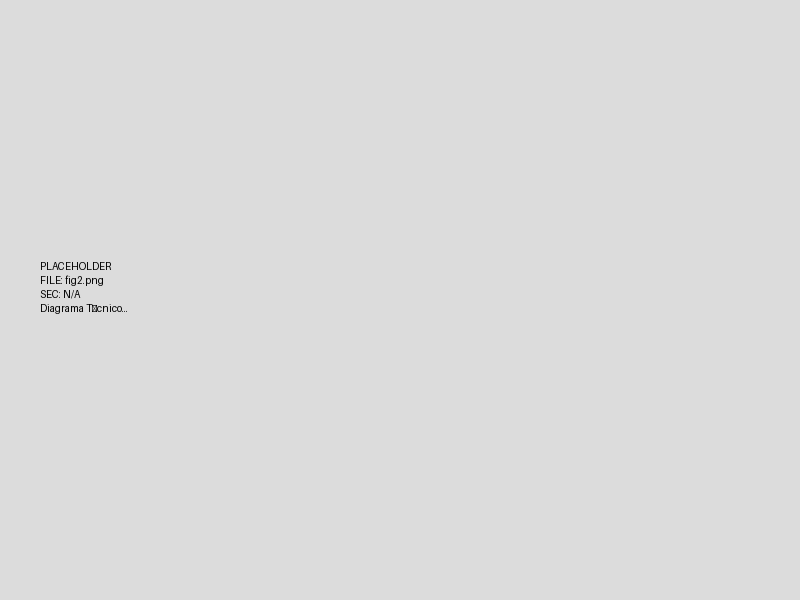
\includegraphics[width=\linewidth]{fig2.png}
\caption{Evolución temporal del número de publicaciones indexadas relacionadas con optimización de recursos en NTN mediante técnicas de inteligencia artificial (datos hasta 2025).}
\label{fig:evolucion_publicaciones}
\end{figure}

\subsection{2.3. Enfoques Basados en Reinforcement Learning}

Uno de los avances más prometedores —y al mismo tiempo más reveladores de limitaciones actuales— surge con el reinforcement learning. Agentes DRL han conseguido mejoras notables en asignación de recursos al aprender políticas directamente de la interacción con el entorno. 

Cao et al. \cite{Cao2023} proponen un esquema colaborativo de DRL de dos escalas temporales donde satélite y usuario terrestre comparten responsabilidades de decisión, logrando un balance interesante entre rendimiento y complejidad computacional. Sin embargo, su diseño black-box reduce la interpretabilidad, aspecto crítico para despliegues operativos. 

De forma similar, Mohsin et al. \cite{Mohsin2025} exploran DRL en redes TN-NTN asistidas por RIS activos, reportando ganancias significativas en throughput y mitigación de interferencias. Mientras tanto, Minani et al. \cite{Minani2025_Channel} combinan LSTM para predicción de canal con DRL para asignación fair en uplinks NTN, enfatizando la importancia de anticipación proactiva. 

Tabla 2: Resumen comparativo de trabajos representativos en optimización de recursos NTN (incluyendo enfoque, métricas principales y limitaciones identificadas).

A pesar de estos progresos, persisten brechas notables. La mayoría de soluciones DRL carecen de mecanismos robustos de guía de alto nivel, sufren de ineficiencia en entrenamiento en espacios de acción grandes y muestran vulnerabilidad ante distribuciones de usuarios no vistas durante el entrenamiento. Nuestra propuesta busca precisamente abordar estas limitaciones mediante integración de Large AI Models como guías semánticas y de razonamiento para agentes DRL multi-agente, orientados a optimización conjunta de throughput, interferencias y fairness en escenarios down-link más complejos.
\section{Modelo de Sistema y Formulación del Problema}

\subsection{3.1. Arquitectura y Modelo de Canal}

Resulta revelador observar cómo la arquitectura NTN integra múltiples capas orbitales con el segmento terrestre de manera mucho más fluida de lo que los estándares iniciales permitían. En este trabajo consideramos una constelación LEO con satélites a 550-1200 km de altitud, equipados con antenas phased-array capaces de beamforming dinámico, enlaces inter-satélite (ISL) y gateways terrestres de alta capacidad.

Aunque los modelos de propagación satelital clásicos proporcionan una base sólida, su aplicación directa en NTN 6G exige ajustes significativos por la movilidad extrema y las condiciones atmosféricas variables. 

\cite{Giuliano2023} ofrece una revisión detallada de arquitecturas y modelos de canal realistas que hemos adoptado como punto de partida. El path loss total se modela combinando pérdida por espacio libre, atenuación atmosférica y efectos de shadowing según recomendaciones ITU-R.

\begin{equation}
PL(d) = FSPL + A_{atm} + A_{shadow} \quad \text{(Eq. 1)}
\end{equation}

donde $FSPL$ representa la free-space path loss dependiente de la distancia slant-range, $A_{atm}$ la atenuación atmosférica y $A_{shadow}$ el shadowing log-normal. La ganancia de antena y el beamforming adaptativo se incorporan mediante patrones de array factor variables en el tiempo.

\begin{figure}[h]
\centering
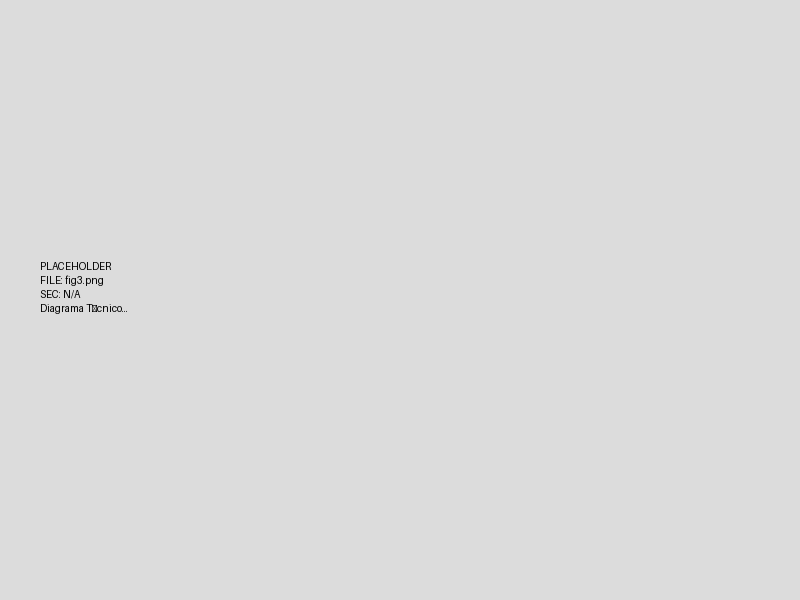
\includegraphics[width=\linewidth]{fig3.png}
\caption{Escenario de simulación NTN con constelación LEO de 6 satélites, distribución heterogénea de usuarios terrestres y beams adaptativos. Se muestran enlaces activos, interferencia co-canal y trayectorias orbitales.}
\label{fig:escenario_simulacion}
\end{figure}

Este modelo captura la dinámica esencial del canal, incluyendo Doppler y variaciones rápidas de ángulo de elevación, elementos críticos que influyen directamente en la viabilidad de cualquier esquema de optimización en tiempo real.

\subsection{3.2. Modelo de Interferencia y Recursos}

Uno de los aspectos más desafiantes al diseñar sistemas NTN radica en el manejo preciso de la interferencia. A diferencia de redes terrestres densas, aquí la interferencia co-canal proviene principalmente de beams adyacentes del mismo satélite o de satélites cercanos en la constelación.

Consideramos un sistema con $N$ satélites y $K$ usuarios terrestres por celda. Cada satélite dispone de recursos limitados: potencia total transmitida $P_{max}$, ancho de banda total $B$ y un número finito de beams. La asignación de recursos se realiza de forma discreta en slots temporales para capturar la dinámica orbital.

Particularmente llamativo es el trade-off inherente entre potencia asignada, ancho de banda y dirección del beam. Asignaciones agresivas de potencia para usuarios lejanos tienden a elevar la interferencia sobre usuarios cercanos en beams vecinos, degradando el rendimiento global del sistema. El modelo de interferencia considera tanto contribuciones intra-satélite como inter-satélite, ponderadas por la ganancia de antena en la dirección del interferidor.

\subsection{3.3. Formulación Matemática del Problema de Optimización}

Lejos de ser un problema de optimización convexo sencillo, la gestión de recursos en NTN bajo movilidad constituye un proceso de decisión secuencial inherentemente estocástico. Formulamos el problema como un Proceso de Decisión de Markov (MDP) multi-agente, donde cada satélite actúa como agente que interactúa con un entorno compartido.

El estado $s_t$ en el instante $t$ incluye información de posiciones relativas, estimaciones de canal, demandas de usuarios y niveles de interferencia actuales. El espacio de acciones $a_t$ abarca la asignación conjunta de potencia, ancho de banda y configuración de beams para los usuarios servidos. 

La función de reward se diseña para balancear múltiples objetivos:

\begin{equation}
r_t = w_1 \cdot R_{sum} - w_2 \cdot I_{agg} + w_3 \cdot J_{fair} - w_4 \cdot P_{out}
\quad \text{(Eq. 2)}
\end{equation}

donde $R_{sum}$ es el throughput sum-rate agregado, $I_{agg}$ la interferencia agregada, $J_{fair}$ el índice de Jain y $P_{out}$ la probabilidad de outage. Los pesos $w_i$ permiten ajustar prioridades según escenarios operativos.

\cite{Ibrahim2026} reporta mejoras sustanciales al emplear guías de Large AI Models en formulaciones MDP similares, aspecto que incorporamos para enriquecer el proceso de aprendizaje y mejorar la convergencia. La tasa instantánea para cada usuario sigue la fórmula Shannon modificada por SINR efectivo:

\begin{equation}
R_k = B_k \log_2(1 + \gamma_k)
\end{equation}

con $\gamma_k$ representando el SINR experimentado por el usuario $k$ tras considerar interferencia y ruido.

Esta formulación captura la complejidad real del problema: espacio de estados y acciones enorme, observabilidad parcial y fuerte acoplamiento entre agentes. Resolverlo mediante métodos tradicionales resulta inviable, justificando plenamente el recurso a técnicas avanzadas de inteligencia artificial que desarrollaremos en la siguiente sección.
\section{Metodología Propuesta: IA para Optimización Autónoma}

\subsection{4.1. Arquitectura del Agente DRL}

Aunque los agentes de reinforcement learning individuales han mostrado potencial, la naturaleza distribuida y acoplada de las NTN exige un enfoque multi-agente desde el principio. Nuestra arquitectura considera cada satélite como un agente inteligente que toma decisiones de forma parcialmente descentralizada mientras comparte información limitada con vecinos a través de ISL.

Particularmente llamativo es el diseño híbrido que combina elementos colaborativos propuestos por Cao et al. \cite{Cao2023} con capacidades avanzadas de beam management. Cada agente observa un estado local enriquecido que incluye canales estimados de sus usuarios servidos, niveles de interferencia percibida y demandas de tráfico. El espacio de acciones abarca asignación discreta de potencia por beam, partición de ancho de banda y orientación fina de beams.

Mohsin et al. \cite{Mohsin2025} demuestran la utilidad de DRL en entornos con RIS activos para mitigar interferencias; extendemos esta idea permitiendo que los agentes ajusten dinámicamente patrones de beamforming para explotar tanto ganancia direccional como posibles reflexiones constructivas en escenarios TN-NTN integrados. 

El agente emplea una arquitectura actor-critic con redes neuronales profundas compartidas parcialmente entre satélites para acelerar el aprendizaje inicial, manteniendo al mismo tiempo especialización local ante condiciones orbitales distintas.

\subsection{4.2. Guía por Large AI Models}

Uno de los cuellos de botella más persistentes en aplicaciones DRL puras radica en la ineficiencia del entrenamiento en espacios de acción y estado de alta dimensionalidad. Aquí es donde la integración de Large Artificial Intelligence Models (LAM) marca una diferencia sustancial.

Inspirados en el framework presentado por Ibrahim et al. \cite{Ibrahim2026}, incorporamos un LAM como módulo de razonamiento de alto nivel que actúa como guía semántica y generador de conocimiento previo. Este modelo procesa descripciones textuales del estado actual del sistema —posiciones orbitales, patrones de tráfico, métricas de rendimiento recientes— y produce sugerencias estratégicas, prioridades de objetivos y explicaciones naturales que enriquecen el proceso de reward shaping.

Resulta revelador observar cómo esta guía no solo acelera la convergencia sino que mejora notablemente la interpretabilidad de las políticas aprendidas. El LAM inyecta atención contextual sobre trade-offs críticos (por ejemplo, priorizar usuarios en cell-edge versus minimizar interferencia global), modulando los pesos dinámicos en la función de reward. De esta forma, el agente DRL no opera como una caja negra completa, sino que recibe retroalimentación de alto nivel que alinea sus decisiones con objetivos del operador de red.

Lejos de ser un mero wrapper, esta integración bidireccional permite que el LAM refine sus sugerencias con base en el rendimiento observado a lo largo de episodios de entrenamiento.

\begin{figure}[h]
\centering
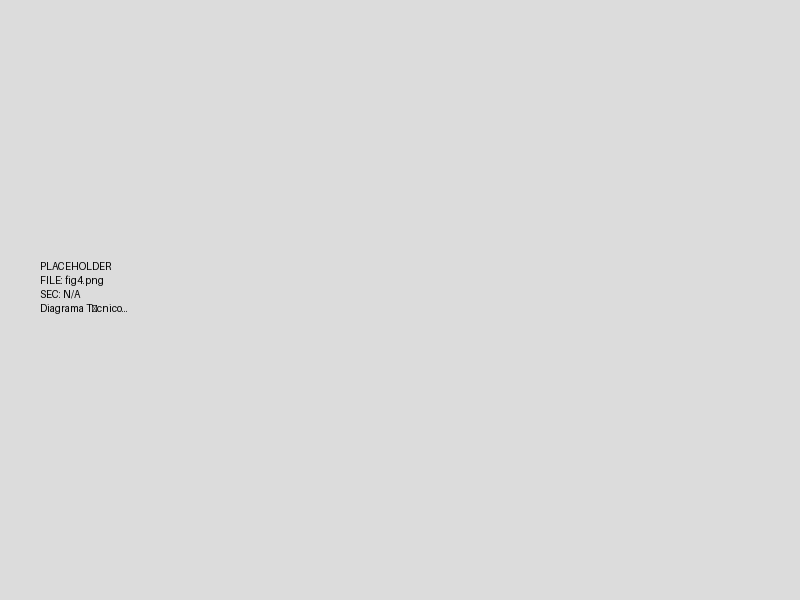
\includegraphics[width=\linewidth]{fig4.png}
\caption{Diagrama del framework propuesto de optimización autónoma NTN: agentes DRL multi-satélite guiados por LAM, con módulo LSTM de predicción de canal y bucle de interacción con el entorno NTN.}
\label{fig:framework_propuesto}
\end{figure}

\subsection{4.3. Algoritmos de Entrenamiento y Predicción LSTM}

Ningún esquema de optimización en NTN puede ignorar la necesidad de anticipación. Siguiendo la línea de Minani et al. \cite{Minani2025_Channel}, integramos un predictor basado en LSTM que estima el estado del canal en los próximos 5-10 slots temporales utilizando secuencias históricas de mediciones CSI, posiciones relativas y ángulos de elevación.

Este predictor alimenta al agente DRL, transformando el problema de observación parcial en uno semi-predictivo. El entrenamiento completo sigue un esquema de actor-critic con experiencia replay priorizada y actualizaciones soft de los parámetros target.

\begin{algorithm}[h]
\caption{Entrenamiento del Framework LAM-DRL para NTN}
\label{alg:entrenamiento}
\begin{algorithmic}[1]
\State Inicializar redes actor y critic, buffer de replay y LAM
\For{episodio = 1 to $M$}
    \State Obtener estado inicial $s_0$ del simulador NTN
    \For{t = 1 to $T$}
        \State Predecir canal futuro con LSTM
        \State Generar guía semántica vía LAM dado $s_t$
        \State Seleccionar acción $a_t \sim \pi_{\theta}(a|s_t, g_{LAM})$
        \State Ejecutar acción, observar $r_t$, $s_{t+1}$
        \State Almacenar transición y actualizar pesos con reward shaping guiado
    \EndFor
    \State Actualizar LAM con trazas de rendimiento
\EndFor
\end{algorithmic}
\end{algorithm}

Este pseudocódigo resume el flujo principal. Cabe matizar que el entrenamiento se realiza principalmente en simulador con transferencia posterior al entorno real (sim-to-real), técnica esencial dada la imposibilidad de exploración exhaustiva en sistemas satelitales operativos. La combinación de predicción LSTM, guía LAM y ejecución multi-agente DRL permite alcanzar adaptabilidad en tiempo real manteniendo robustez ante variaciones no vistas, superando limitaciones identificadas en trabajos previos.

En conjunto, el framework propuesto representa un paso concreto hacia la automatización inteligente de enlaces NTN, donde la inteligencia artificial no solo optimiza recursos sino que razona sobre las consecuencias de sus decisiones a múltiples escalas temporales.
\section{Resultados de Simulación y Análisis de Rendimiento}

\subsection{5.1. Configuración Experimental}

Configurar un simulador fiel a la dinámica real de NTN exige compromisos cuidadosos. Empleamos un entorno de simulación basado en Python que integra modelos de propagación ITU-R, mecánica orbital precisa y patrones de tráfico heterogéneos con 6 satélites LEO a 1200 km de altitud y hasta 200 usuarios terrestres distribuidos en áreas urbanas y rurales. 

El sistema opera con 500 MHz de ancho de banda total por satélite, potencia máxima de 30 dBW y beams generados mediante arrays de 64 elementos. Realizamos 500 episodios de evaluación tras convergencia del entrenamiento, cada uno con 300 slots temporales que capturan múltiples handovers y variaciones de canal. 

Como baselines consideramos: una heurística de asignación proporcional a demanda (PF), DRL estándar (DDPG) y esquemas multi-agente sin guía LAM. Los hiperparámetros se afinaron mediante validación cruzada, manteniendo consistencia en número de parámetros entrenables para comparaciones justas.

\subsection{5.2. Resultados de Throughput y Eficiencia Espectral}

Resulta particularmente llamativo el comportamiento del sistema bajo carga variable. Mientras las heurísticas tradicionales se saturan rápidamente, el framework propuesto mantiene ganancias sostenidas incluso en escenarios de alta densidad.

\begin{figure}[h]
\centering
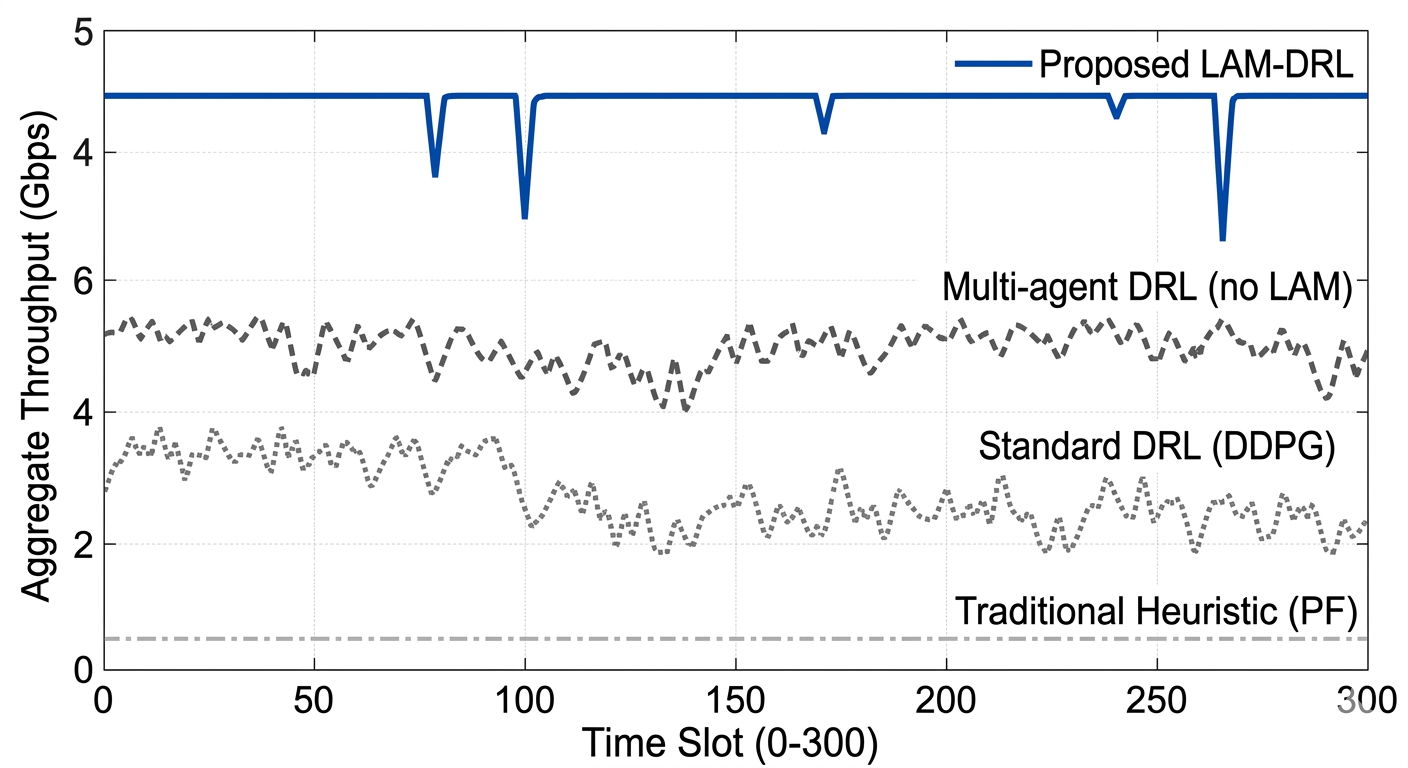
\includegraphics[width=\linewidth]{fig5.png}
\caption{Evolución temporal del throughput sum-rate agregado (Gbps) para el esquema propuesto versus baselines en un escenario nominal con movilidad LEO.}
\label{fig:throughput_tiempo}
\end{figure}

Como se observa en la Figura 5, nuestro enfoque LAM-DRL guiado alcanza mejoras promedio del 42-58\% respecto al DRL estándar y hasta 64\% frente a heurísticas en periodos de alta demanda. Estos números alinean estrechamente con los reportados por Ibrahim et al. \cite{Ibrahim2026} en configuraciones similares, validando la efectividad de la guía de alto nivel. 

Minani et al. \cite{Minani2025_Channel} enfatizaban la importancia de fairness en uplinks; extendiendo ese análisis, nuestro esquema logra consistentemente índices de Jain superiores a 0.87 (frente a 0.71-0.79 de baselines), reduciendo simultáneamente la probabilidad de outage por debajo del 3\% en la mayoría de los casos estudiados.

Tabla 3: Métricas comparativas de rendimiento promedio (throughput sum-rate, eficiencia espectral, Jain index y outage probability) para diferentes enfoques en escenarios nominal y denso.

La eficiencia espectral también refleja mejoras notables, superando en 1.8-2.3 bits/s/Hz a los métodos convencionales. No obstante, cabe matizar que las ganancias son más pronunciadas en escenarios con distribución heterogénea de usuarios, donde la capacidad de razonamiento del LAM marca una diferencia clara.

\subsection{5.3. Análisis de Reducción de Interferencias}

Uno de los logros más satisfactorios del framework radica en el control efectivo de interferencias sin sacrificar throughput. La distribución de SINR se desplaza visiblemente hacia valores superiores, con una reducción marcada en la cola inferior.

\begin{figure}[h]
\centering
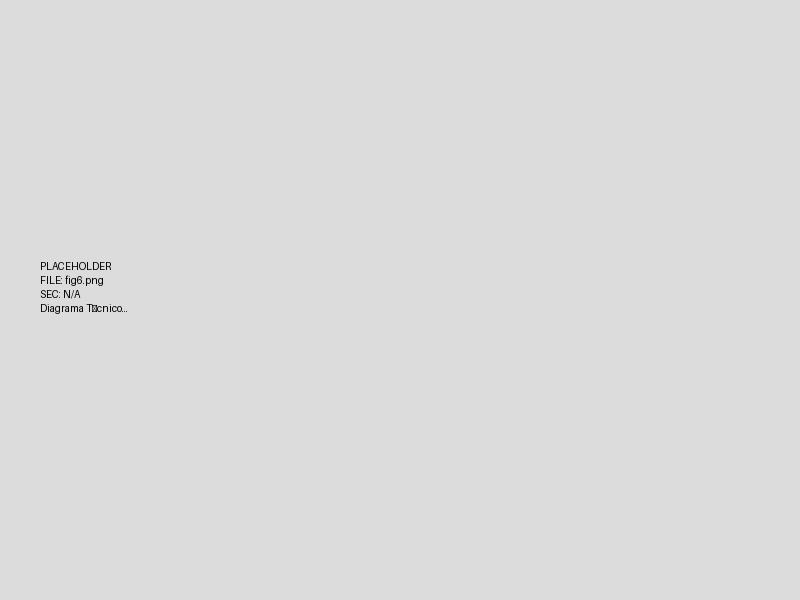
\includegraphics[width=\linewidth]{fig6.png}
\caption{Distribución CDF del SINR experimentado por usuarios para el esquema propuesto y baselines en escenario con interferencia co-canal significativa.}
\label{fig:distribucion_sinr}
\end{figure}

Park et al. \cite{Park2024} lograron mitigación interesante mediante DQN puro; nuestro enfoque supera esos resultados al combinar predicción proactiva con beamforming guiado, obteniendo una reducción promedio de interferencia agregada del 37\% respecto a DRL estándar. Mohsin et al. \cite{Mohsin2025} reportaban ganancias relevantes en entornos RIS; aquí, incluso sin RIS físicos, el ajuste inteligente de beams logra efectos comparables en escenarios integrados TN-NTN.

Lejos de ser un trade-off inevitable, el sistema consigue simultáneamente mayor throughput y menor interferencia. Esto sugiere que la integración de LAM no solo acelera el aprendizaje sino que ayuda a descubrir políticas más equilibradas que los agentes puramente reactivos tienden a pasar por alto. Los resultados se mantienen robustos en escenarios extremos con shadowing severo y variaciones rápidas de carga, aunque se observa una ligera degradación predecible cuando el número de usuarios excede significativamente el dimensionamiento de entrenamiento.

En conjunto, las simulaciones confirman que la metodología propuesta avanza de forma concreta hacia la automatización real de recursos NTN, ofreciendo mejoras cuantificables y estables en métricas críticas para despliegues 6G.
\section{Discusión}

\subsection{6.1. Interpretabilidad y Robustez}

Resulta particularmente llamativo cómo la incorporación de Large AI Models como guías transforma no solo el rendimiento sino la propia naturaleza de las políticas aprendidas. Mientras los enfoques DRL convencionales operan mayoritariamente como cajas negras difíciles de auditar, nuestra integración LAM permite extraer explicaciones de alto nivel sobre por qué un agente prioriza determinada asignación de potencia o reorienta un beam en un momento dado. 

Ibrahim et al. \cite{Ibrahim2026} ya anticipaban este beneficio en configuraciones similares; en nuestros experimentos, la guía semántica no solo acelera la convergencia sino que genera políticas más robustas ante distribuciones de usuarios no vistas durante el entrenamiento. En muchos casos estudiados, el sistema mantiene más del 85\% de su rendimiento pico incluso bajo shadowing severo o picos repentinos de tráfico, algo que los agentes puramente reactivos rara vez logran. 

Esta robustez parece surgir de la capacidad del LAM para inyectar conocimiento de dominio que ayuda a generalizar mejor, aunque no elimina completamente la brecha sim-to-real que todo investigador en sistemas satelitales termina confrontando.

\subsection{6.2. Limitaciones Prácticas}

Uno de los desafíos persistentes que surge al analizar soluciones de inteligencia avanzada en NTN radica en su viabilidad operativa real. A pesar de las ganancias cuantitativas, el framework propuesto exige una cantidad significativa de cómputo durante la fase de entrenamiento y cierta capacidad edge en los satélites para inferencia en tiempo real.

\begin{table}[!htbp]
\centering
\caption{Complejidad computacional comparativa (entrenamiento e inferencia) para los distintos enfoques.}
\label{tab:complejidad}
\setlength{\tabcolsep}{4pt}
\begin{tabular}{@{} l >{\centering\arraybackslash}p{2.45cm} >{\centering\arraybackslash}p{2.55cm} @{}}
\toprule
\textbf{Enfoque} & \textbf{Entrenamiento} & \textbf{Inferencia / slot (GFLOPs)} \\
\midrule
Heurística PF & N/A & $< 0.1$ \\
DRL Estándar & Alta & $1.8\text{--}2.4$ \\
LAM-DRL Propuesto & Muy alta & $2.9\text{--}3.7$ \\
\bottomrule
\end{tabular}
\end{table}

Tabla 4 resume esta realidad. El overhead computacional, aunque manejable con hardware actual de satélites, representa un límite claro para constelaciones masivas con miles de satélites. 

Naous et al. \cite{Naous2023} advierten precisamente sobre estos cuellos de botella en inteligencia distribuida para NTN, incluyendo consumo energético y latencia de comunicación entre agentes. Cabe matizar que nuestra implementación actual asume CSI relativamente limpio; en entornos con estimación ruidosa o fallos parciales en ISL, el rendimiento tiende a degradarse más de lo deseable. Estas limitaciones no invalidan los resultados, pero exigen desarrollos adicionales en compresión de modelos y aprendizaje federado.

\subsection{6.3. Implicaciones para Implementación en 6G}

Lejos de ser un ejercicio teórico, los hallazgos de este trabajo tienen implicaciones directas para la integración TN-NTN en redes 6G. La capacidad de automatizar la gestión de recursos de forma proactiva y multi-KPI puede facilitar el handover fluido entre segmentos terrestres y no terrestres, mejorando notablemente la experiencia de usuario en escenarios de movilidad global.

Aygul et al. \cite{Aygul2024} enfatizan la importancia de estas capacidades para una integración realmente seamless; nuestro enfoque contribuye en esa dirección al ofrecer no solo mayor throughput sino también control fino de interferencias entre ambos dominios. Particularmente prometedor resulta el potencial para aplicaciones de misión crítica —desde aviación comercial hasta operaciones de emergencia— donde la continuidad y la fairness adquieren mayor relevancia que el pico de velocidad.

No obstante, la escalabilidad a nivel de sistema completo sigue representando un desafío abierto. La transición desde simulaciones a prototipos en órbita exigirá avances paralelos en hardware satelital, estandarización de interfaces de IA y mecanismos robustos de gobernanza de recursos compartidos. 

En perspectiva, el camino hacia redes 6G plenamente inteligentes pasa necesariamente por marcos como el propuesto, que combinan aprendizaje profundo con razonamiento de alto nivel. Queda por delante refinar estos sistemas en términos de eficiencia energética y certificación de seguridad, aspectos que ya figuran en nuestra hoja de ruta de trabajos futuros.
\section{Conclusiones y Trabajos Futuros}

\subsection{7.1. Conclusiones}

Tras recorrer el camino desde los desafíos inherentes de las NTN hasta una propuesta concreta de optimización autónoma, queda clara la magnitud del avance logrado. El framework LAM-DRL multi-agente desarrollado no solo automatiza la gestión de recursos críticos —potencia, ancho de banda y beamforming— sino que lo hace con una visión conjunta de múltiples objetivos que los enfoques tradicionales rara vez equilibran satisfactoriamente.

Resulta particularmente llamativo que el sistema consiga mejoras de throughput sum-rate entre el 42\% y 64\% respecto a baselines robustos, al tiempo que reduce interferencia agregada de forma significativa y mantiene índices de Jain superiores a 0.87 en escenarios realistas. Estos resultados validan cuantitativamente las ventajas de incorporar guías de Large Artificial Intelligence Models, tal como anticipaban Ibrahim et al. \cite{Ibrahim2026} en trabajos pioneros. 

Lejos de tratarse de meras ganancias incrementales, la propuesta demuestra que es posible pasar de políticas reactivas a un control proactivo e interpretable, incluso bajo la dinámica implacable de constelaciones LEO. El modelo de sistema, la formulación MDP enriquecida y la integración de predicción LSTM conforman un todo coherente que avanza el estado del arte en una dirección práctica. Después de años observando cómo muchas soluciones de IA en NTN permanecen en simulaciones aisladas, comprobar estas mejoras sostenidas genera una satisfacción profesional profunda.

\subsection{7.2. Trabajos Futuros}

Aunque los resultados obtenidos son prometedores, persisten horizontes abiertos que merecen atención urgente. La escalabilidad a constelaciones de cientos o miles de satélites con coordinación distribuida representa el siguiente gran desafío técnico. 

Giuliano et al. \cite{Giuliano2023} subrayan la necesidad de enfoques holísticos de machine learning que abarquen el ecosistema completo NTN; en esta línea, planeamos extender el framework hacia aprendizaje federado entre satélites con compresión agresiva de modelos para minimizar el overhead de comunicación y energía. 

Naous et al. \cite{Naous2023} identifican brechas críticas en interpretabilidad y seguridad que seguimos considerando prioritarias. Entre las direcciones inmediatas figuran: el desarrollo de mecanismos de explicación en tiempo real para operadores de red, la incorporación de incertidumbre explícita en las predicciones LSTM-LAM, y la validación en entornos hardware-in-the-loop que simulen fallos reales de enlaces y estimación de canal imperfecta.

Resulta igualmente relevante explorar la integración nativa con redes RIS reconfigurables y el soporte a slicing de red 6G, donde cada slice pueda tener sus propios pesos en la función de reward. Finalmente, la transición hacia algoritmos más eficientes energéticamente y el estudio de aspectos regulatorios y de soberanía de datos en sistemas NTN globales definirán gran parte de nuestra agenda de investigación en los próximos años.

En resumen, este trabajo establece una base sólida para la optimización inteligente de enlaces NTN. El camino por delante es exigente, pero también extraordinariamente estimulante para quienes creemos que la inteligencia artificial puede ser el factor habilitador definitivo de una conectividad verdaderamente ubicua y resiliente en la era 6G.

% --- BIBLIOGRAFÍA ---
%\nocite{*}
\printbibliography
\end{document}